
% Document class options:
% =======================
% blind: Anonymise all author, affiliation, correspondence
%        and funding information.
%
% lineno: Adds line numbers.
%
% serif: Sets the body font to be serif. 
%
% twocolumn: Sets the body text in two-column layout. 
% 
% num-refs: Uses numerical citation and references style 
%           (Vancouver-authoryear).
%
% alpha-refs: Uses author-year citation and references style
%             (rss).
%
% Using other bibliography styles:
% =======================
%
% To specify a different bibiography style
%
% 1) Do not use either num-refs or alpha-refs in documentclass.
% 2) Load natbib package with the options set as needed.
% 3) Use the \bibliographystyle command to specify the style
% 
% Included NJD styles are: 
%   WileyNJD-ACS
%   WileyNJD-AMA
%   WileyNJD-AMS
%   WileyNJD-APA
%   WileyNJD-Harvard
%   WileyNJD-VANCOUVER
%
% or you may upload an alternative .bst file 
% (if requested by the journal).
%
% Examples:
% =======================
%% Example: Using numerical, sort-by-authors citations.
\documentclass[authordate, serif, review]{jote-article}


\usepackage{latexsym}
\usepackage[normalem]{ulem}
\usepackage{soul}
\usepackage{array}
\usepackage{extarrows}
\usepackage{graphicx}

\usepackage{subfig}
\usepackage{wrapfig}
\usepackage{enumitem}
\usepackage{adjustbox}
\usepackage{longtable}
\usepackage{changepage}
\usepackage{setspace}
\usepackage{hhline}
\usepackage{multicol}
\usepackage{tabto}
\usepackage{multirow}
\usepackage{fancyhdr}
%\usepackage[toc,page]{appendix}

\usepackage{flowchart}
%\usepackage[paperheight=11.0in,paperwidth=8.5in,left=0.5in,right=0.5in,top=1.0in,bottom=1.0in,headheight=1in]{geometry}
\usepackage[utf8]{inputenc}
\usepackage[T1]{fontenc}
\usepackage{csquotes}


%\addbibresource{julie.bib}


%% Example: Using author-year citations and anonymising submission
% \documentclass[blind,alpha-refs]{wiley-article}

%% Example: Using unsrtnat for numerical, in-sequence citations
% \documentclass{wiley-article}
% \usepackage[numbers]{natbib}
% \bibliographystyle{unsrtnat}

%% Example: Using WileyNJD-AMA reference style and superscript
%%          citations, two-column and serif fonts for AIChE
% \documentclass[serif,twocolumn,lineno]{wiley-article}
% \usepackage[super]{natbib}
% \bibliographystyle{WileyNJD-AMA}
% \makeatletter
% \renewcommand{\@biblabel}[1]{#1.}
% \makeatother

% Add additional packages here if required
\usepackage{siunitx}


\usepackage{float}
\usepackage{bookmark}
\usepackage{lipsum}
% Update article type if known
% Include section in journal if known, otherwise delete
\papertype{Empirical}

\title{Alcohol Cues and Their Effects on Sexually Aggressive Thoughts}

% List abbreviations here, if any. Please note that it is preferred that abbreviations be defined at the first instance they appear in the text, rather than creating an abbreviations list.
%\abbrevs{ABC, a black cat; DEF, doesn't ever fret; GHI, goes home immediately.}

% Include full author names and degrees, when required by the journal.
% Use the \authfn to add symbols for additional footnotes and present addresses, if any. Usually start with 1 for notes about author contributions; then continuing with 2 etc if any author has a different present address.

%Please also enter the authors in the same order here, for metadata purposes. This is a workaround.

\author[1]{Alexa Ruel} 
\author[2]{Jeremy Ullman}
%\authorfour{}
%\authorfive{}

%\contrib[\authfn{1}]{Equally contributing authors.}

% Include full affiliation details for all authors
\affil[1]{Reviewer 1}
\affil[2]{Reviewer 2}

\ogauthor{Julie Leboeuf, Stine Linden-Anderson, Jonathan Carriere}
\prround{1}
%\affil[2]{Department, Institution, City, State or Province, Postal Code, Country}

\corraddress{Julie Leboeuf, Department of Psychology, Bishop's University, Sherbrooke, Quebec, J1M 1Z7, Canada}
\corremail{jleboeuf16@ubishops.ca}

%\presentadd[\authfn{2}]{Department, Institution, City, State or Province, Postal Code, Country}

\paperdoi{10.36850/e1}

% Include the name of the author that should appear in the running header
\runningauthor{Leboeuf et al.}

\jname{Journal of Trial and Error}
\jyear{2020}
%\jvolume{Fall}
\jwebsite{https://jtrialerror.com}
%\paperrevised{May 18th 2020}
\paperpublished{2 December, 2020}
\paperpublisheddate{2020-12-2}
%\jpages{1-12}
\jlogo{media/jote_logo_full}



%\keywords{alcohol, automatic cognition, gender stereotypes, lexical decision task, sexual aggression}

%\abstracttext{Alcohol and its effects on aggression have been the subject of many discussions and research papers. Despite this fact, there is still a debate surrounding what it is exactly about alcohol that causes aggression. The current study sought to replicate the past finding by Bartholow \& Heinz (2006), that alcohol cues without consumption increase the accessibility of aggressive thoughts, which can then influence aggressive behaviors. In the present study, participants had to complete a lexical decision task that was set up to assess whether aggressive words were detected faster in the presence of alcohol-related pictures compared to neutral pictures. The results of this study did not replicate the expected finding as only a main effect of word type was found in which participants detected neutral words faster than aggressive words. Furthermore, the study aimed to assess the role of gender stereotype acceptance levels in this association, but due to faulty design considerations, such analyses were not possible. The results are discussed in terms of the limitations of the study, and propositions for future directions are addressed.}


\heightabstract{70mm}
\widthaffil{65mm}

\setlength{\parskip}{0pt}

%\contributions{\lipsum[1]}

\keywordsabstract{alcohol, automatic cognition, gender stereotypes, lexical decision task, sexual aggression}


\begin{document}
\begin{frontmatter}
\maketitle

\begin{abstract}
%\phantomsection
%\addcontentsline{toc}{section}{Abstract}

\noindent Alcohol and its effects on aggression has been the subject of many discussions and research papers. Despite this fact, there is still a debate surrounding what it is exactly about alcohol that causes aggression. The current study sought to replicate the past finding by Bartholow and Heinz (2006) that alcohol cues without consumption increase the accessibility of aggressive thoughts, which can then influence aggressive behaviors. In the present study, participants had to complete a lexical decision task that was set up to assess whether aggressive words were detected faster in the presence of alcohol-related pictures compared to neutral pictures. The results of this study did not replicate the expected finding as only a main effect of word type was found in which participants detected neutral words faster than aggressive words. Furthermore, the study was trying to assess the role of gender stereotype acceptance levels in this association, but no significant result was found, meaning that one's degree of endorsement of societal expectations about genders did not influence reactions times in the lexical decision task. The results are discussed in terms of the limitations of the study, and propositions for future directions are addressed.

% Please include a maximum of seven keywords
\end{abstract}
\end{frontmatter}

\begin{multicols}{2}
\phantomsection
\addcontentsline{toc}{section}{Take Home Message}
\section*{Take Home Message} \gotoreview
\label{sec:take-home}

\noindent The present study failed to replicate the finding by Bartholow and Heinz (2006) that alcohol cues without consumption increase the accessibility of aggressive thoughts. This failure to replicate can mainly be explained by a flawed sample; the small size reduced statistical power, and the different composition of the sample compared to the original study impacted the ability to recreate the results.  

\phantomsection
\addcontentsline{toc}{section}{Introduction}
\section*{Introduction} \gotoreview
\label{sec:introduction}

\noindent In many parts of the world, alcohol consumption is quite frequent in festive contexts. Indeed, adults typically enjoy consuming alcoholic beverages when it comes to social events, or simply to relax. Despite the benefits that alcohol consumption might appear to have, it must be kept in mind that it also comes with its negatives. According to the World Health Organization (2018), harmful use of alcohol results in 3 million deaths worldwide every year. Furthermore, Field, Caetano, and Nelson (2004) found that among all the factors under investigation, what appeared to be the strongest predictor of intimate partner violence was the expectations of aggressive behavior following alcohol consumption. Although the pharmacological effects of alcohol have been well researched (Chermack \& Taylor, 1995; Giancola, 2000; Heinz, Beck, Meyer-Lindenberg, Sterzer, \& Heinz, 2001), there is less information available with regards to other factors, such as cognitions and expectancies, that can lead to aggression in alcohol-related contexts. Bartholow and Heinz (2006) as well as Subra, Muller, Bègue, Bushman, and Delmas (2010) researched whether simple exposure to alcohol-related cues unconsciously increases the availability of aggressive thoughts, thus increasing the possibility of aggressive behaviors. In both studies the researchers found that participants made faster lexical decisions when aggression-related words were paired with alcohol-related pictures compared with neutral primes.  

Before exploring more thoroughly the body of research pertaining to automatic aggressive cognitions associated with sheer exposure to alcohol cues, it is worthwhile to mention that similar studies have examined how other stimuli can generate aggressive thoughts. In 1998, Anderson, Benjamin, and Bartholow reported that simple identification of weapon primes was linked to an increase in aggressive thoughts. The authors further argued that this increase resulted from the weapon stimuli automatically priming aggression-related thoughts (1998). More specifically, the authors refer to the semantic network model of memory which posits that words or concepts that are similar in meaning or that repeatedly co-occur together are activated simultaneously in the semantic memory and therefore develop strong associations. This model goes as far as to propose that this increase in aggressive thoughts subsequently increases the likelihood that these thoughts will affect behavior (Bartholow \& Heinz, 2006). 

While weapons have been reported to be linked with an increase in aggression-related thoughts, other elements from the environment that could similarly influence levels of aggressive thoughts, such as alcohol, should also be considered. Although it is a generally accepted premise that alcohol increases aggression, there is still a debate as to what exactly causes or explains this increase (Bartholow \& Heinz, 2006), and it is usually best explained through a combination of theories and viewpoints (see Heinz et al., 2001 for a comprehensive review). Some leading theories are first that the increased aggression results from the physiological disinhibition produced by alcohol intake; second, that it is best explained through expectancy effects; and third, that it is indirectly caused as alcohol consumption produces changes at the cognitive and emotional levels which then increase the likelihood of aggressive acts being committed (Bushman, 2002). Briefly stated, the physiological disinhibition hypothesis states that alcohol intake increases the levels of aggression by anesthetizing the part of our brain that usually keeps our aggressive impulses under control, making people more likely to express aggressive behaviors (2002). Following the same line of reasoning, the indirect cause explanation proposes that alcohol consumption might increase aggression levels by enacting changes into people that further allow for the possibility of aggressive acts being committed, such as by affecting one's intellectual functioning and reducing one's self-awareness (2002). As for the expectancy hypothesis, it holds that alcohol is linked with aggression because people expect it to be that way (2002). This presumed effect/expectancy hypothesis suggests that people tend to associate aggression and alcohol together, even if only unconscious, which potentially accounts for one of the ways in which alcohol consumption is linked with aggression (Batholow \& Heinz, 2006). The problem with this hypothesis is that evidence supporting it mostly comes from placebo designs, which makes it is unclear whether a belief that alcohol consumption has occurred is necessary for this unconscious association to be activated, or whether the presence of alcohol cues alone can increase the accessibility of aggressive thoughts (2006).  

To address this methodological limitation, Bartholow and Heinz (2006) conducted a study in which they examined the extent to which alcohol cues without consumption or belief that alcohol has been consumed (i.e., placebo effect) could increase the accessibility of aggressive thoughts. They tested 121 undergraduate students, and they had them participate in a lexical decision task. The participants were first primed with a stimulus and were then shown a string of letters, and they had to decide whether the letter string presented to them was a legitimate English word. The priming stimuli could either be alcohol-related pictures, weapon-related pictures, or neutral images, and the letter string could either represent aggression-related words, neutral words, or nonwords. In this experiment, the neutral images consisted of plants, and the weapon pictures were included to create a reference point by allowing comparison with the results showing a link between weapon exposure and aggressive thoughts obtained by Anderson, Benjamin, and Bartholow (1998). Results showed that participants identified aggression-related words faster when exposed to aggression-related pictures compared with neutral images. 

In 2010, Subra et al. replicated the study by Bartholow and Heinz with a different population as well as by including a slight methodological modification. First, their study was conducted with a French-speaking population as opposed to an English one, and the sample was not restricted to undergraduate students. Subra and his colleagues used the same stimuli as those used by the authors of the 2006 study, but they used different images for the neutral condition. They criticized the ones previously used by Bartholow and Heinz on the basis that their nature (i.e. plants) was not neutral since nature scenes have been shown to decrease aggressive thoughts (Kuo \& Sullivan, 2001a, 2001b). Instead, they used photos displaying non-alcoholic beverages for their neutral condition. Similarly to the study under replication, participants made faster lexical decisions about aggression-related words when exposed to alcohol or weapon primes compared with neutral primes.  

The two studies by Bartholow and Heinz (2006) and Subra et al. (2010) suggest that exposure to alcohol cues without consumption is linked with an increase in aggression-related thoughts. Interestingly, the target words that were used for the aggression category were mainly of a physical nature (e.g., punch, assault, murder) and did not assess sexual violence. It would be worth investigating whether this increase in thoughts of an aggressive nature also extends to sexual violence, especially when considering that the World Health Organization (n.d.) listed the use of alcohol or drugs as a factor that increases the risk of men committing rape, and that severe alcohol intoxication is implicated in almost half of all sexual aggression cases worldwide (Testa, 2002). Additionally, past research has shown that alcohol priming without consumption can increase sexual expectancies. Friedman, McCarthy, Förster, and Denzler (2005) reported that men who were exposed to suboptimal alcohol-related words rated women as being more sexually attractive, and that this effect was more precisely caused by the sexual expectancies associated with alcohol intake. It does not seem too farfetched to assume that similar effects could be found with sexual violence. To demonstrate how severe the problem of unwanted touching and sexual aggressions can be in alcohol settings such as bars and clubs, an online article titled ``Touch-sensitive dress reveals staggering level of sexual harassment at clubs'' reported about an experiment conducted by the ad agency Ogilvy in which three women were ask to wear a touch-sensitive dress to a nightclub in Brazil. The authors recorded how many times women were touched or groped in the span of three hours and 47 minutes; the final number came to 157 times, and the principal areas where women were being touched included the waist, buttocks and thighs (Hignett, 2018). 

Another element that was not assessed in the 2006 and 2010 studies is gender stereotypes acceptance. In one study, Abbey (2002) reported that traditional gender roles beliefs about dating and sexuality could be at play in explaining the occurrence of sexual assaults, no matter whether alcohol was involved or not. More precisely, endorsing such beliefs as interpreting a woman's refusal as an invitation to be convinced, or that forced sex is sometimes acceptable, was a proposed factor that could increase the likelihood of sexual assault being committed. While recognizing that this is a good first step into assessing the role of gender stereotypes acceptance with regards to sexual violence, it seems that more general gender role beliefs should be investigated to truly understand the function that gender stereotypes plays in sexual violence occurrences. To this effect, Locke and Mahalik (2005) reported that men who showed a problematic use of alcohol and who conformed to such masculine norms as having power over women and being violent were more inclined to score higher on the Rape Myth Acceptance Scale and to report more sexually aggressive behaviors. The first study mentioned here only looked at gender stereotypes with regards to sexuality and dating (Abbey, 2002), and although this second study by Locke and Mahalik (2005) might seem to assess gender stereotypes more generally, it appears biased towards specific stereotypes with regards to power dynamics between men and women. Another problem with the literature on gender stereotype beliefs and its relationship to violence is that the vast majority of the articles available only report about men committing sexually violent behaviors, or on the relationship between men's level of gender stereotypes and the perpetration of violent acts, thus leaving women out of the picture (Jakupcak, Lisak, \& Roemer, 2005; Gidycz, Warkentin, \& Orchowski, 2007; Abbey, Clinton-Sherrod, McAuslan, Zawacki, \& Buck 2003). There is a clear need to investigate the relationship between gender stereotype beliefs and sexual violence as it relates not only to men, but to women as well.  

\phantomsection
\addcontentsline{toc}{section}{Objective and Hypotheses}
\section*{Objective and Hypotheses}

The objective of this project is to further the line of research on the effects of alcohol cues on aggressive behaviors by testing this relationship specifically with sexually aggressive words and by taking into account gender stereotype beliefs. More precisely, the aggressive words used by Bartholow and Heinz (2006) will be replaced by aggressive words of a sexual nature. There was a discussion about keeping half of the original words and only replacing the other half by sexually aggressive words, but for statistical power purposes, it was better to substitute all the original physically aggressive words for sexually aggressive words. Therefore, the comparison point will be against the two studies that have investigated this before and for which significant results have been reported, namely the one by Bartholow and Heinz (2006) and the one by Subra et al. (2010). Gender stereotypes acceptance will be evaluated through the German Extended Personal Attributes Questionnaire (Runge, Frey, Gollwitzer, Helmreich, \& Spence, 1981). 

It is hypothesized that participants will make faster lexical decisions to aggressive words of a sexual nature when paired with alcohol-related primes compared with neutral primes. A similar effect should also be found with the weapon-related primes. Furthermore, it is suggested that for both men and women this association will likely be different depending on one's level of gender stereotypes acceptance. Indeed, results are expected to show a non-significant association at low levels of gender stereotypes beliefs, a moderate interaction at medium levels of gender stereotype beliefs, and a dramatically significant interaction at high levels of gender stereotype beliefs. Finally, for replication purposes, it is expected that participants will be slightly more accurate at identifying neutral words compared to aggressive words.  

\phantomsection
\addcontentsline{toc}{section}{Methods}
\section*{Methods} \gotoreview
\label{sec:methods}
\phantomsection
\addcontentsline{toc}{subsection}{Participants}
\subsection*{Participants}
Sixty participants took part in this study, but two of them were excluded from the analyses, giving a final sample size of 58. One participant was excluded because the experiment failed before the data could be recorded, and the other participant was excluded because it was clear from the debriefing session that this participant had not understood the computer task properly, and their accuracy rate was only 66%.  

From the remaining participants, 49 self-identified as women (84.5\%) and nine as men (15.5\%). No one expressed a mismatched between their sex at birth and gender identified with, and no one selected the `other' option for their self-identified gender. The age of the participants ranged between 18 years old and 46 years old ($M = 21.64$, $SD = 7.71$) and they were all enrolled at Bishop's University. Different programs were represented, but most participants (65.5\%) were majoring in psychology.  

\subsection*{Stimuli and Task}
\addcontentsline{toc}{subsection}{Stimuli and Task}
\textbf{Questionnaires.} In this experiment two different questionnaires were used: a short demographic questionnaire and the German Extended Personal Attributes Questionnaire, a scale evaluating gender stereotype acceptance and beliefs (Runge, Frey, Gollwitzer, Helmreich, \& Spence, 1981). This questionnaire includes two subscales both comprising eight items, namely ``expressivity'' and ``instrumentality'', which are intended to measure the degree to which someone can be classified according to masculine (i.e., instrumentality subscale) or feminine (i.e., expressivity subscale) adjectives. Therefore, the questionnaire constitutes of 16 semantic differential scale items ranging from 1 to 5, and sample items include ``\textit{Not independent -- Very independent}''  and ``\textit{Not emotional -- Very emotional}'' (see Appendix A and B for complete questionnaires). In its original form, this questionnaire was designed to assess self-ascribed masculinity or femininity, but for the purpose of this study, it was modified to assess one's view and degree of endorsement of gender stereotypes in general. To that end, participants were asked to indicate to what extent they believe that the sixteen characteristics are representative of men in general, and they were then asked to fill out the questionnaire a second time, but this time by indicating to what extent they believe that the said characteristics are generally representative of women.  

To facilitate the analyses, the German Extended Personal Attributes Questionnaire was scored differently than how it was originally conceived to b. Total scores were calculated for each participant, and participants were classified as belonging to one of three groups reflecting of their level of gender stereotypes acceptance: low, medium, and high. Each item is rated on a 5-point semantic differential scale; a score of 3 (middle of the scale) was given a value of 0, scores of 2 or 4 were given a value of 1, and scores of 4 or 5 (extremes of the scale) were given a value of 2. With 32 items in the questionnaire, and a maximum of 2 points per question, the total scores could range between 0 and 64. Instead of using pre-established cut-off points for the groups, participants were divided into 3 equal groups using the visual binning option is SPSS.  

\textbf{Task.} Participants had to complete a lexical decision task in which they had to decide whether a string of letters presented to them was a legitimate English word. Prime stimuli consisted of fifteen photos: five containing alcohol bottles, five portraying weapons, and five showing non-alcoholic beverages (see Figure 1 for sample pictures). Target words were also divided into three categories, each containing 15 words (see Appendix C for the complete list): aggression-related words of a sexual nature (e.g., grope, rape), neutral words (e.g., observe, vanish), and nonword letter strings (e.g., wenct, jork). Each photo was paired with 3 aggressive words, 3 non-aggressive words, and 3 nonword letter strings for a total of 135 trials. For each trial, an image was presented for 300ms, followed by a 200ms interval prior to the showing of the target word, which stayed on the screen until the participants responded or up to 3 seconds. Participants had to indicate by pressing on a key whether the letters formed a legitimate English word or not. An interval of 3 seconds separated each trial.

\phantomsection
\addcontentsline{toc}{subsection}{Procedures}
\subsection*{Procedures}

Participants were asked to come to the Psychological Health and Well-Being lab on the Bishop's University campus for one session lasting between 30 minutes and 45 minutes. They were first presented with a consent form and were instructed to carefully read it and to vocalize any questions they might have. Following the procedure by Barthlow and Heinz (2006), partial disclosure was used in that participants were told that the goal of the experiment was to measure the speed of language comprehension in the presence of distractive information (i.e., pictures). Once they had agreed to participate in the study, they were asked to complete two different paper questionnaires, including a short demographic questionnaire and a questionnaire pertaining to gender stereotype acceptance levels (GSAL), as mentioned above. 

Next, participants were asked to complete the main task of the study, which is the computer-based lexical decision task described above. After completion of the lexical decision task, debriefing took place; participants were informed of the reasons justifying the use of partial disclosure, and a new consent form was presented to them. If they had wished not to renew their consent, their questionnaires would have been shredded and their computer data electronically destroyed. However, this was not an issue since no participant decided to remove their data from the study. Furthermore, they were invited to provide their email address in order to enter a draw to win a \$50 gift card of their choice. Lastly, participants were given a list of psychological resources, and any questions and/or concerns were addressed before they left the laboratory.

\phantomsection
\addcontentsline{toc}{section}{Results}
\section*{Results} \gotoreview
\label{sec:results}

\noindent Following the procedure used by Bartholow and Heinz (2006), trials on which the participants' response times (RTs) where smaller than 150ms or greater than 1,500ms where deleted and excluded from analyses (less than 3\% of all trials). Furthermore, response times to nonwords were not included in the analyses because they were only used in the study for methodological reasons and do not have any bearing on the present hypotheses being tested (Bartholow \& Heinz, 2006). The data from the demographic questionnaire was not used in the analyses for different reasons. First, since there was no discrepancy between gender identified with and sex at birth, no comparison was possible in that case. Next, given that there was only nine men in the study, the sample size was not large enough to run analyses based on gender differences. Finally, considering that everyone was enrolled at Bishop's University, no comparison could have been done, and field of study was not used either but will be mentioned later in the discussion.   

\phantomsection
\addcontentsline{toc}{subsection}{Response Times}
\subsection*{Response Times}

Only the correct-response trials were kept for the response times analyses. That is, the trials where participants misidentified a nonword for a word, and vice-versa, were excluded from the present analyses (less than 5\% of the remaining trials). The mean response times values did not show any skewness and did not need to be corrected through a log transformation, contrary to what the two groups of authors had previously found (2006, 2010). The reaction times were analyzed using a 3 (prime type: weapon-related pictures, alcohol-related pictures, neutral pictures) x 2 (target word type: aggression-related words, neutral words) x 3 (gender stereotype acceptance levels: low, medium, high) repeated measures analysis of variance (ANOVA), and the sphericity assumption was not violated in any of the analyses; therefore, the statistics reported are the original ones. Main effects of prime type, target word type, and gender stereotypes acceptance levels are presented in Table 1. The main effect of target word type was significant, $F (1, 55) = 148.589$, $p < .001$. More precisely, neutral words were detected faster ($M = 600ms$, $SE = 13ms$) than aggressive words ($M = 657ms$, $SE = 13ms$). This main effect goes against the expected results. Indeed, Bartholow and Heinz (2006) and Subra et al. (2010) had both found a main effect of word type as well, except that it went into the other direction, meaning that aggressive words were detected faster than neutral words. All the other main effects were not statistically significant and neither were the interactions. The expected main effect of prime type was not significant ($F (2, 110) = 1.186$, $p = .309$), and the interaction between prime type and target word type also did not reach the significance level ($F (2, 110) = 0.025$, $p = .975$). This also goes against the past literature where the authors had found both stated analyses to be significant (2006, 2010). Although not relevant to the hypotheses, the two-way interactions between prime type and GSAL and between target word type and GSAL were not significant ($F (4, 110) = 0.556$, $p = .695$; $F (2, 55) = 0.156$, $p = .856$, respectively). Finally, the additional hypothesis about gender stereotype acceptance levels was not supported as indicated by the lack of significance of the three-way interaction between prime type, target word type and GSAL ($F (4, 110) = 1.532$, $p = .198$).

\phantomsection
\addcontentsline{toc}{subsection}{Accuracy}
\subsection*{Accuracy}

The analyses performed for the accuracy levels are identical to those performed for reaction times, except that the trials on which the participants made a wrong decision were not excluded. Mean accuracy values did not show any kurtosis and did not need to be corrected through an arcsine transformation, contrary to the main study being replicated (Bartholow \& Heinz, 2006). The overall accuracy level was 95\%, but this variable was further analyzed and broken down through a 3 (prime type: weapon-related pictures, alcohol-related pictures, neutral pictures) x 2 (target word type: aggression-related words, neutral words) x 3 (gender stereotype acceptance levels: low, medium, high) repeated measures (ANOVA), and again, the sphericity assumption was never violated. Replicating the results by Bartholow and Heinz (2006) and Subra et al. (2010), the main effect of target word type was significant, $F (1, 55) = 45.591$, $p < .001$. More precisely, neutral words were detected with more accurately ($M = .98$, $SE = .003$) than aggressive words ($M = .919$, $SE = .010$). All the other main effects were not statistically significant and neither were the interactions, which supports the hypothesis. The main effect of prime type was not significant ($F (2, 110) = 0.101$, $p = .904$), and the interaction between prime type and target word type also did not reach the significance level ($F (2, 110) = 0.088$, $p = .916$). Therefore, the results found cannot be attributed to a speed-accuracy trade-off.  Although not relevant to the hypothesis, the two-way interactions between prime type and GSAL and between target word type and GSAL were not significant ($F (4, 110) = 0.589$, $p = .671$; $F (2, 55) = 0.440$, $p = .646$, respectively). Finally, the three-way ANOVA between prime type, target type and GSAL did not reach statistical significance either ($F (4, 110) = 0.629$, $p = .643$). 


\phantomsection
\addcontentsline{toc}{subsection}{Gender Stereotypes Acceptance Levels}
\subsection*{Gender Stereotypes Acceptance Levels}

This section is devoted to describing the characteristics of the participants in the three obtained GSAL groups. As was mentioned before, participants were divided into the three groups based on relative cut-off points instead of pre-established ones. In the first group, the total scores obtained on the questionnaire ranged from 7 to 20, in the second group from 21 to 28, and in the third group, from 28 to 52. The first group, low on GSAL, consisted of 22 participants (18 woman, 81.8\%), with a mean age of 20.68 years old ($SD = 2.01$), and 14 of them (63.6\%) were enrolled in psychology. The second group, medium on GSAL, consisted of 18 participants (16 women, 88.9\%), with a mean age of 22.83 years old ($SD = 7.67$), and 11 (61.1\%) were majoring in psychology. Finally, the third group, high on GSAL, consisted of 18 participants (15 women, 83.3\%), with a mean age of 21.61 years old ($SD = 2.81$), and 13 (66.7\%) had listed psychology as their major. At first glance, the groups do not seem to differ significantly on the mentioned characteristics, but no analyses were run on this specifically.

\phantomsection
\addcontentsline{toc}{section}{Discussion}
\section*{Discussion} \gotoreview
\label{sec:discussion}

\noindent Contrary to what Bartholow and Heinz (2006) and Subra et al. (2010) had previously reported, the results obtained in this study do not support the hypothesis that alcohol cues increase the accessibility of aggressive thoughts. Whereas they had found that aggressive words were detected faster when preceded by alcohol or weapon pictures compared to neutral pictures, and that aggressive words were detected faster than neutral words, none of those results were replicated in the present study. Indeed, there was no significant difference in the rapidity of detection of aggressive words across the different types of pictures, and neutral words, as opposed to aggressive ones, were recognized faster by the participants. However, the finding by both groups of authors that neutral words are detected with more accuracy was replicated in this study, but this has no importance for the hypotheses. Finally, the unique hypothesis that was added to this study with regards to gender stereotype acceptance levels and their expected influence on response times was also not supported.  

\phantomsection
\addcontentsline{toc}{subsection}{Limitations}
\subsection*{Limitations}
The sample of participants in this study was problematic on many levels. First, when dealing with response times and differences in terms of milliseconds, it usually takes a large sample size to maximize statistical power. A sample size of 58 participants was probably not large enough to optimize statistical power, especially when compared the 121 participants that were recruited by Bartholow and Heinz (2006). Furthermore, whereas they had recruited 60 men and 61 women, the present study included 49 women and 9 men. This difference in men-women proportion is problematic considering that past studies reporting a link between drinking and aggression have focused on the perpetration of aggressive acts by men, and not women (Jakupcak, Lisak, \& Roemer, 2005; Gidycz, Warkentin, \& Orchowski, 2007; Abbey, Clinton-Sherrod, McAuslan, Zawacki, \& Buck 2003; Locke \& Mahalik, 2005). It is therefore plausible that a greater proportion of men in the current student would have led to different results. However, this still does not explain why the main effect of target word type found in this study contradicted the ones that both previous studies reported; no effect would have been easier to understand than a contradictory effect. Another problem with the current sample is its lack of generalizability. Undergraduate samples do not represent the general population, but this was not so much a concern for this research project as the population of interest was university students. However, what is more problematic is the lack of men representation, and the overrepresentation of psychology students. The composition of this sample is not representative of the general university population, and although it might not entirely explain the failure to replicate past findings, it is important to keep this issue in mind when looking at the results.  

Another major limitation of this study relates to the word choice for the aggressive target word type category. Finding aggressive words of a sexual nature proved to be challenging for many different reasons. One of them is that most of the words that could be found through internet searches were expressions made up of more than one word and could not be used as word length has an impact on reaction times (Bartholow \& Heinz, 2006). Another problem that came up is that the line between sexually aggressive words and sexual preferences is somewhat blurry (e.g., sodomy, choke); therefore, some of the words used might not have been associated with violence for certain participants but with pleasure instead. Finally, the face value of some of the words in the aggressive category was doubtful, the best example being the use of the word `prey'. Thus, it is likely that the results of this study might have been negatively impacted by the flawed word choice for the aggressive target word type category.  

The images used for the neutral prime and the alcohol-related prime represent another important limitation to the present study. Some of the images that were used contained words in them, such as `Corona' being written on the beer bottles, or again `Nesquik' as could be seen on a chocolate milk bottle. During the debriefing session, some participants reported finding it difficult and confusing to assess the letter strings when they were preceded by a photo on which there was some writing. Another point that was brought up by some participants is that the neutral pictures may have been more effective if they had not been beverages. The argument is that it becomes too obvious that the study is researching the effects of alcohol as it is contrasted with non-alcoholic beverages, despite the fact that weapon pictures are also included. As mentioned earlier, the reason brought forward by Subra et al. (2010) for choosing non-alcoholic beverages pictures was to address the limitation to Bartholow and Heinz' study (2006). The conclusion from this is that neither plants nor non-alcoholic beverages are an optimal neutral category for this study and that the ideal neutral prime has yet to be found.  

The German Extended Personal Attributes Questionnaire came with its own set of limitations. Namely, there seemed to be a bias in the participant's answers as most of the participants tended to `sit on the fence' -- that is, they gravitated towards the middle and shied away from the extremes. The questions is whether the participants purposely answered towards the middle because of social desirability or if those answers reflected their true attitudes towards women and men in general. However, some of the items on the questionnaire are obvious at face value which may have made the participants answer in a socially desirable way. For example, a lot of participants changed their answers on the first part of the questionnaire when they got to the second part. This was observed by the investigator while participants were answering the questionnaire, and can also be seen by the number of scribbles and changed answers on the sheets. Another difficulty related to the questionnaire was with its coding. Since it was used differently than its original conception, the same coding strategy could not be applied. It is debatable whether the right way of categorizing people into groups was selected, and it is even blurrier whether the questionnaire was effective in accessing gender stereotype acceptance levels all together. Finally, the decision to divide people into equal groups instead of classifying them according to pre-established cut-off points was perhaps not the most efficient way to go about. The problem is that participants did not answer in the extremes enough, and using pre-established cut-offs points would have classified most people falling into the second group, making it impossible to run proper statistical analyses. Briefly stated, the items on the questionnaire might have been too obvious at face value which may have made people answer in a socially desirable way, the method of coding was unclear, and the way in which participants were divided into the three gender stereotype acceptance levels groups was not representative of true GSAL.  

\phantomsection
\addcontentsline{toc}{subsection}{Future Directions }
\subsection*{Future Directions }

The limitations listed previously can be used to help guide future directions. A larger and more representative sample would be necessary if this study was to be tried again. Secondly, the sexually aggressive words would need to be revisited, and perhaps a manipulation check could be done to test the face value of the words before including them in the study. Next, the images used in the three categories should be selected taking into consideration that writing on the pictures might be distracting, and the neutral category of pictures should be changed to something that does not involve beverages of any kind, such as furniture or bags. Finally, the questionnaire should either be changed completely, or the issue of coding should be explored in more depth as to maximize the questionnaire's efficiency.  

 Another aspect that would be interesting to investigate in future studies would be to inquire about nationality to see if the patterns of response times would be different depending on one's nationality. This idea emerged during the debriefing sessions as multiple participants reported coming from Europe and being raised with an open-minded attitude towards alcohol, and some also said that sexual violence was not necessarily associated with alcohol for them. One of them main studies that was under replication, that by Subra et al. (2010) did take place in France, but it was investigating the link between alcohol and physical violence as opposed to sexual violence. Therefore, it would be worthwhile to investigate whether participants with a European nationality have different patterns of responses when it comes to alcohol and sexual violence compared to people of a Canadian nationality, and even more interesting would be to include both sexually aggressive words and physically aggressive words in the study to explore more directly the possible difference in response times patterns.  

Another avenue that would be worth investigating is the relationship between aggressive thoughts and subsequent behavior. Right now, the studies by Bartholow and Heinz (2006) and Subra et al. (2010) point to the fact that alcohol-related cues can increase the accessibility of aggressive thoughts. How does this translate into behavior, if it does so at all? Bartholow and Heinz (2006) did follow up on their first experiment with a second one, which was not under replication, aimed at investigating the effects of this increase in aggressive thoughts, but they only showed that it was related to more aggressive interpretations of the behavior of others, and did not assess whether the participants would also be more likely to commit aggressive acts (2010)  A direct link between an increase in aggressive thoughts and a subsequent increase in aggressive behaviors should be strongly established by research; however, how to conduct this kind of experiment in an ethical manner remains to be answered. 

\phantomsection
\addcontentsline{toc}{section}{Conclusion}
\section*{Conclusion} \gotoreview
\label{sec:conclusion}

\noindent This current research project was undertaken to extend the literature by replicating the evidence that simple exposure to alcohol stimuli without actual consumption or belief that consumption has occurred can increase aggressive thoughts. The initial intention of this project was always to complete a replication of the first of the two experiments by Bartholow and Heinz (2006) with new data, which implies keeping the same protocol as the original study while collecting new data (NWO, 2019). Conveniently enough, Dr. Bartholow provided me with the original target word stimuli and with a description of the images used in his study. However, since different aggressive words were used and a variable (GSAL) was added, it can be argued that the current research project would fall under the category of replication with the same research question, which is defined by new data collection and a new research protocol with the same research question (2019). I disagree; the initial research protocol was followed closely and the research question remained unchanged. The added questionnaires can be regarded as an additional investigation that could be part of a second experiment altogether; remove those questionnaires, and it becomes clear that the original research protocol was respected, even if the nature of the aggressive words was altered. The main problems encountered during this replication study were getting an appropriate number of participants and getting enough men to partake in the study. This low number of participants might be explained by the timing of testing, which occurred close to the end of the academic semester at Bishop's University. It is possible that a more optimal testing period would have increased the total number of participants, but it remains unclear why so few men participated. Another impediment to replication might have been the alteration of the aggressive target words since it is doubtful whether the new words were of a similar relevance than the original ones. 

In conclusion, although the present study failed to replicate the previous finding that alcohol-related cues increase the accessibility of aggressive thoughts (Bartholow \& Heinz, 2006; Subra et al., 2010), it does not mean that the effect is non-existent. Rather, it is probable that the methodology employed in this study was significantly flawed and reduced the likelihood of finding significant differences in the variables. This line of research should be further pursued as it bears significant importance on today's society.  

% \setlength{\bibhang}{\parindent}
% \nocite{*} 
% \phantomsection
% \addcontentsline{toc}{section}{References}
% \printbibliography

\newpage

\phantomsection
\addcontentsline{toc}{section}{Peer Reviews}
\section*{Peer Reviews}
\label{sec:reviews}

\noindent \begin{reviewend}{ Alexa Ruel}
    \begin{enumerate}[label=\textbf{\arabic*}), start=0]
    \item \textbf{General comments}
        \begin{enumerate}
            \item This is an interesting non-replication of a study previously showing that alcohol cues without consumption increase the accessibility of aggressive thoughts, which can then influence aggressive behaviors. The authors of the current manuscript attempted to replicate this 2006 study and extend the findings by examining the role of gender stereotype.
            \item Below are many comments, but few require major changes. Thus, I suggest the paper get the note of revise \& resubmit.
            \item Sufficiently detailed autopsy? For the most part, the author included a sufficiently exhaustive list of limitations on the current study. Additional comments are made in-text.
            \item Add additional reflections on why the project failed: The biggest faults in this project appear to be design-related. While statistical significance and effect size are related to sample size, the choices regarding the structure of the lexical decision trials and the choices for stimuli in the materials lists (both visual and lexical) jump out as red flags above and beyond gripes with the sample characteristics.
        \end{enumerate}

    \item \hyperref[sec:introduction]{Introduction}
        \begin{enumerate}
            \item $[...]$ reasoning between substituting physically aggressive words for sexually aggressive is unnecessary. 
            \item  Why do the authors predict that their findings would be in line with the original study? This needs to be clearly motivated.
        \end{enumerate}


    \item \hyperref[sec:methods]{Methods}
        \begin{enumerate}
            \item The performance of the subject excluded due to failing to understand the task instructions should be compared to chance. If the subject did not understand, it should not be statistically different from chance performance on the task.

            \item $[...]$ The other majors should be reported as well in addition to the 65\% psychology. 

            \item Typo on [p. 3] ``than how it was originally conceived to b''.
            
            \item $[$p. 4$]$  ``If they had wished not to renew their consent, their questionnaires would have been shredded and their computer data electronically destroyed. However, this was not an issue since no participant decided to remove their data from the study. Furthermore, they were invited to provide their email address in order to enter a draw to win a \$50 gift card of their choice. Lastly, participants were given a list of psychological resources, and any questions and/or concerns were addressed before they left the laboratory.'' This is not necessary; to be removed.
            
        \end{enumerate}

    \item \hyperref[sec:results]{Results}
        \begin{enumerate}
            \item Some of the statistical analyses seem to have been done incorrectly. If the authors found no significant 3-way interaction effect, further 2-way interactions should not be analysed. This is to be removed from the results and discussion (``the two-way interactions between prime type and GSAL and between target word type and GSAL'').
            \item `Gender Stereotype Acceptance Levels' section should go before the Response time analyses. 
            \item No need to include the majors in the gender for stereotype acceptance levels section [...]
        \end{enumerate}
        
    \item \hyperref[sec:conclusion]{Conclusion}
        \begin{itemize}
            \item  Regarding the optimal testing period: in my personal experience, it is not just the number of students seeking to participate in studies that changes but also the \textit{quality} of participants declines toward the end of the semester. More importantly, the testing period doesn't feel like a limitation, as more participants can always be collected with more time. Having \textit{n} participants is the same whether they were all collected the same day or over a few weeks.
        \end{itemize}
    \end{enumerate}
    
%    \tcbsubtitle{Editor}
%    \begin{itemize}
%    \item
%    \end{itemize}
\end{reviewend}

\newpage

\begin{reviewend}{ Jeremy Ullman}
    \begin{enumerate}[label=\textbf{\arabic*}), start=0]
        \item \textbf{General comments}
            \begin{itemize}
                \item Alcohol consumption pervades many social and cultural contexts, but its benefits are often outweighed by its drawbacks. The consequences of alcohol consumption can be deadly; it has the power to end relationships and lives. The effects of alcohol cues on consumption and consumption on (aggressive) behavior are discussed in light of a handful of theories. These span the physiological (ex. disinhibition) to the psychological (ex. expectancy). The current study picks up where previous studies, which look at different types of cues, have left off. One goal is to shift focus towards gender stereotyping and sexual violence in relation to alcohol and aggression. Participants filled out a number of questionnaires that were modified to fit the current research question. As well, a lexical decision task with various images (alcohol, violence, neutral) and letter strings (neutral, violent, non-words) were presented. The study attempts and fails to replicate the results of Bartholow \& Heinz (2006) and Subra et al. (2010) that exposure to alcohol cues without consumption elicits aggressive thoughts.
            \end{itemize}
            
        \item \hyperref[sec:take-home]{Take home message}
            \begin{itemize}
                \item I think the overall design considerations (or lack thereof) should be mentioned as one of the main explanations of the failure to replicate the findings, as opposed to sample-related issues only.
            \end{itemize}
            
        \item \hyperref[sec:introduction]{Introduction}
            \begin{itemize}
                \item Opening line could be stronger. ``In many parts of the world, alcohol consumption is quite frequent in festive contexts'' is a bit of a vague statement and lacks the attention-grabbing nature of a truly enticing hook. Using words like \textit{quite }and\textit{ typically} in your openings sentences can wash out the strength of your statements. Alternatively, opening with the line that begins ``According to the World Health Organization{\dots}'' is considerably more eye-catching, while slyly dodging overt sensationalism.
            \end{itemize}
            
        \item \hyperref[sec:methods]{Methods}
            \begin{enumerate}
                \item The interstimulus latencies on the lexical decision task were too long. 
                \item It is likely that the questionnaires were manipulated and modified to a point where their results would be uninterpretable. Unfortunately, questionnaires are not one-size-fits-all.
            \end{enumerate}
            
        \item \hyperref[sec:results]{Results}
            \begin{itemize}
                \item Regarding the opening line of this section: if you are giving a 300ms prime + 200ms pause after the prime then how can you accept a response under 500ms, let alone 150ms? Technically all responses under 500ms should be scrapped because of this, since participants would have not even had time to see the target.
            \end{itemize}
    \end{enumerate}
    % \tcbsubtitle{Editor}
    % \begin{itemize}
    %     \item 
    % \end{itemize}
\end{reviewend}

\newpage
\end{multicols}
%\onecolumn
\phantomsection
\addcontentsline{toc}{Section}{Appendices}
\section*{Appendices}
\phantomsection
\addcontentsline{toc}{subsection}{Table 1}
\subsection*{\hypertarget{table1}{Table 1}}
\textit{Main Effects of Prime Type and Target Type}
%%%%%%%%%%%%%%%%%%%% Table No: 1 starts here %%%%%%%%%%%%%%%%%%%%
\begin{table}[H]
 \centering
\begin{tabular}{p{2.69in}p{0.4in}p{0.49in}}
\hline
%row no:1
\multicolumn{1}{|p{2.69in}}{Variable} & 
\multicolumn{1}{|p{0.4in}}{\Centering \textit{M}} & 
\multicolumn{1}{|p{0.49in}|}{\Centering \textit{SE}} \\
\hhline{---}
%row no:2
\multicolumn{1}{|p{2.69in}}{Prime type} & 
\multicolumn{1}{|p{0.4in}}{} & 
\multicolumn{1}{|p{0.49in}|}{} \\
\hhline{---}
%row no:3
\multicolumn{1}{|p{2.69in}}{Weapon-related pictures} & 
\multicolumn{1}{|p{0.4in}}{\Centering 625} & 
\multicolumn{1}{|p{0.49in}|}{\Centering 13} \\
\hhline{---}
%row no:4
\multicolumn{1}{|p{2.69in}}{Alcohol-related pictures} & 
\multicolumn{1}{|p{0.4in}}{\Centering 628} & 
\multicolumn{1}{|p{0.49in}|}{\Centering 13} \\
\hhline{---}
%row no:5
\multicolumn{1}{|p{2.69in}}{Neutral pictures} & 
\multicolumn{1}{|p{0.4in}}{\Centering 633} & 
\multicolumn{1}{|p{0.49in}|}{\Centering 13} \\
\hhline{---}
%row no:6
\multicolumn{1}{|p{2.69in}}{Target word type} & 
\multicolumn{1}{|p{0.4in}}{} & 
\multicolumn{1}{|p{0.49in}|}{} \\
\hhline{---}
%row no:7
\multicolumn{1}{|p{2.69in}}{Sexually aggressive words} & 
\multicolumn{1}{|p{0.4in}}{\Centering 657} & 
\multicolumn{1}{|p{0.49in}|}{\Centering 13} \\
\hhline{---}
%row no:8
\multicolumn{1}{|p{2.69in}}{Neutral words} & 
\multicolumn{1}{|p{0.4in}}{\Centering 600} & 
\multicolumn{1}{|p{0.49in}|}{\Centering 13} \\
\hhline{---}
\end{tabular}
\end{table}
%%%%%%%%%%%%%%%%%%%% Table No: 1 ends here %%%%%%%%%%%%%%%%%%%%
\begin{adjustwidth}{0.49in}{0.0in}
\textit{Note}. All the reaction times depicted in the table are presented in milliseconds (ms).\  
\end{adjustwidth}
%%%%%%%%%%%%%%%%%%%% Figure/Image No: 1 starts here %%%%%%%%%%%%%%%%%%%%
\begin{figure}[H]
	\centering
	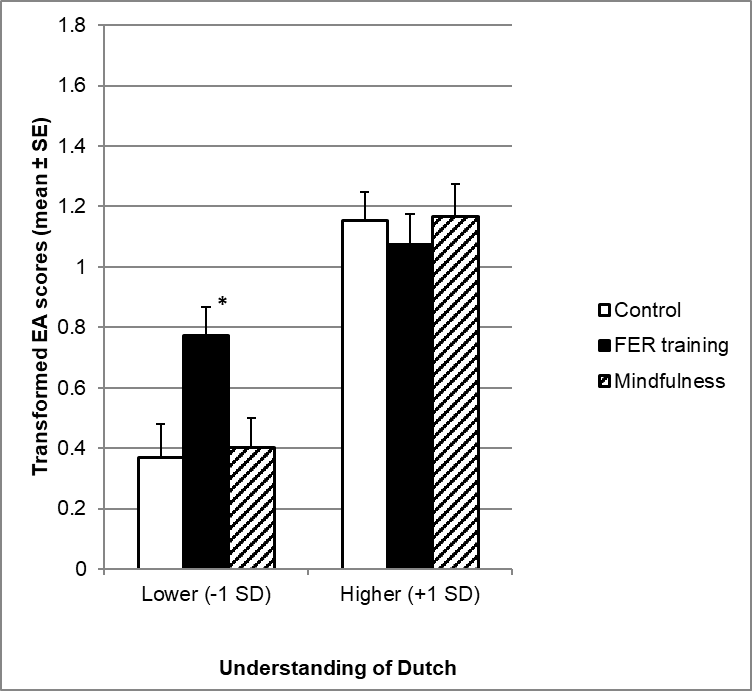
\includegraphics[scale=0.7]{media/image1.png}
	\caption{Alcohol-related picture examples (a, b), weapon-related picture examples (c, d), and neutral picture examples (e, f).}
\end{figure}
%%%%%%%%%%%%%%%%%%%% Figure/Image No: 1 Ends here %%%%%%%%%%%%%%%%%%%
\newpage

\subsection*{\hypertarget{A}{Appendix A}} 
\addcontentsline{toc}{subsection}{Appendix A}
\begin{Center}
Field of Study -- Complete List
\end{Center}
%%%%%%%%%%%%%%%%%%%% Table No: 2 starts here %%%%%%%%%%%%%%%%%%%%
\begin{table}[H]
 			\centering
\begin{tabular}{p{1.6in}p{1.6in}} 
\hline
%row no:1
\multicolumn{1}{|p{1.3in}}{\Centering Field of study} & 
\multicolumn{1}{|p{1.3in}|}{\Centering \textit{n}} \\
\hhline{--}
%row no:2
\multicolumn{1}{|p{1.3in}}{Psychology} & 
\multicolumn{1}{|p{1.3in}|}{\Centering 38} \\
\hhline{--}
%row no:3
\multicolumn{1}{|p{1.3in}}{Biology} & 
\multicolumn{1}{|p{1.3in}|}{\Centering 4} \\
\hhline{--}
%row no:4
\multicolumn{1}{|p{1.3in}}{Languages} & 
\multicolumn{1}{|p{1.3in}|}{\Centering 3} \\
\hhline{--}
%row no:5
\multicolumn{1}{|p{1.3in}}{Education} & 
\multicolumn{1}{|p{1.3in}|}{\Centering 2} \\
\hhline{--}
%row no:6
\multicolumn{1}{|p{1.3in}}{Sociology} & 
\multicolumn{1}{|p{1.3in}|}{\Centering 2} \\
\hhline{--}
%row no:7
\multicolumn{1}{|p{1.3in}}{Physics} & 
\multicolumn{1}{|p{1.3in}|}{\Centering 1} \\
\hhline{--}
%row no:8
\multicolumn{1}{|p{1.3in}}{Politic Sciences} & 
\multicolumn{1}{|p{1.3in}|}{\Centering 1} \\
\hhline{--}
%row no:9
\multicolumn{1}{|p{1.3in}}{Biochemistry} & 
\multicolumn{1}{|p{1.3in}|}{\Centering 1} \\
\hhline{--}
%row no:10
\multicolumn{1}{|p{1.3in}}{History} & 
\multicolumn{1}{|p{1.3in}|}{\Centering 1} \\
\hhline{--}
%row no:11
\multicolumn{1}{|p{1.3in}}{English Literature} & 
\multicolumn{1}{|p{1.3in}|}{\Centering 1} \\
\hhline{--}
%row no:12
\multicolumn{1}{|p{1.3in}}{Mathematics} & 
\multicolumn{1}{|p{1.3in}|}{\Centering 1} \\
\hhline{--}
%row no:13
\multicolumn{1}{|p{1.3in}}{Finance} & 
\multicolumn{1}{|p{1.3in}|}{\Centering 1} \\
\hhline{--}
%row no:14
\multicolumn{1}{|p{1.3in}}{Arts Administrations} & 
\multicolumn{1}{|p{1.3in}|}{\Centering 1} \\
\hhline{--}
%row no:15
\multicolumn{1}{|p{1.3in}}{Sports Studies } & 
\multicolumn{1}{|p{1.3in}|}{\Centering 1} \\
\hhline{--}

\end{tabular}
 \end{table}

%%%%%%%%%%%%%%%%%%%% Table No: 2 ends here %%%%%%%%%%%%%%%%%%%%

\phantomsection
\addcontentsline{toc}{subsection}{Appendix B}
\subsection*{\hypertarget{B}{Appendix B}} 
\begin{Center}

\end{Center}
%%%%%%%%%%%%%%%%%%%% Figure/Image No: 2 starts here %%%%%%%%%%%%%%%%%%%%
\begin{figure}[H]
	\centering
	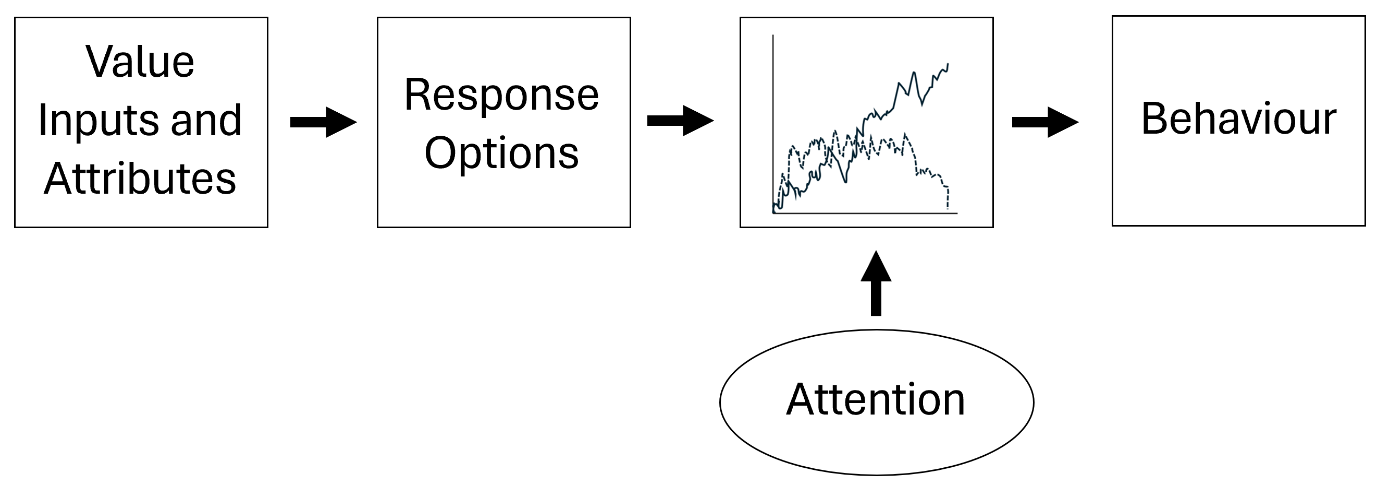
\includegraphics[width=5.54in,height=2.01in]{media/image2.png}
\end{figure}
%%%%%%%%%%%%%%%%%%%% Figure/Image No: 2 Ends here %%%%%%%%%%%%%%%%%%%%

\newpage
\phantomsection
\addcontentsline{toc}{subsection}{Appendix C}
\subsection*{\hypertarget{C}{Appendix C}}

\begin{Center}
German Extended Personal Attributes Questionnaire
\end{Center}

In general, I see \textbf{MEN} as being:



%%%%%%%%%%%%%%%%%%%% Table No: 3 starts here %%%%%%%%%%%%%%%%%%%%



%\setlength\extrarowheight{3pt}
\begin{longtable}{p{1.6in}p{0.2in}p{0.2in}p{0.2in}p{0.2in}p{0.2in}p{1.6in}}

\endfirsthead

\endfoot
\endlastfoot\hline
%row no:1
\multicolumn{1}{|p{1.6in}}{Not independent} & 
\multicolumn{1}{|p{0.2in}}{\textit{1}} & 
\multicolumn{1}{|p{0.2in}}{\textit{2}} & 
\multicolumn{1}{|p{0.2in}}{\textit{3}} & 
\multicolumn{1}{|p{0.2in}}{\textit{4}} & 
\multicolumn{1}{|p{0.2in}}{\textit{5}} & 
\multicolumn{1}{|p{1.6in}|}{Very independent} \\
\hhline{-------}
%row no:2
\multicolumn{1}{|p{1.6in}}{Very passive} & 
\multicolumn{1}{|p{0.2in}}{\textit{1}} & 
\multicolumn{1}{|p{0.2in}}{\textit{2}} & 
\multicolumn{1}{|p{0.2in}}{\textit{3}} & 
\multicolumn{1}{|p{0.2in}}{\textit{4}} & 
\multicolumn{1}{|p{0.2in}}{\textit{5}} & 
\multicolumn{1}{|p{1.6in}|}{Very active} \\
\hhline{-------}
%row no:3
\multicolumn{1}{|p{1.6in}}{Not competitive} & 
\multicolumn{1}{|p{0.2in}}{\textit{1}} & 
\multicolumn{1}{|p{0.2in}}{\textit{2}} & 
\multicolumn{1}{|p{0.2in}}{\textit{3}} & 
\multicolumn{1}{|p{0.2in}}{\textit{4}} & 
\multicolumn{1}{|p{0.2in}}{\textit{5}} & 
\multicolumn{1}{|p{1.6in}|}{Very competitive} \\
\hhline{-------}
%row no:4
\multicolumn{1}{|p{1.6in}}{Decisive} & 
\multicolumn{1}{|p{0.2in}}{\textit{1}} & 
\multicolumn{1}{|p{0.2in}}{\textit{2}} & 
\multicolumn{1}{|p{0.2in}}{\textit{3}} & 
\multicolumn{1}{|p{0.2in}}{\textit{4}} & 
\multicolumn{1}{|p{0.2in}}{\textit{5}} & 
\multicolumn{1}{|p{1.6in}|}{Not decisive} \\
\hhline{-------}
%row no:5
\multicolumn{1}{|p{1.6in}}{Gives up easily} & 
\multicolumn{1}{|p{0.2in}}{\textit{1}} & 
\multicolumn{1}{|p{0.2in}}{\textit{2}} & 
\multicolumn{1}{|p{0.2in}}{\textit{3}} & 
\multicolumn{1}{|p{0.2in}}{\textit{4}} & 
\multicolumn{1}{|p{0.2in}}{\textit{5}} & 
\multicolumn{1}{|p{1.6in}|}{Never gives up} \\
\hhline{-------}
%row no:6
\multicolumn{1}{|p{1.6in}}{Not self-confident} & 
\multicolumn{1}{|p{0.2in}}{\textit{1}} & 
\multicolumn{1}{|p{0.2in}}{\textit{2}} & 
\multicolumn{1}{|p{0.2in}}{\textit{3}} & 
\multicolumn{1}{|p{0.2in}}{\textit{4}} & 
\multicolumn{1}{|p{0.2in}}{\textit{5}} & 
\multicolumn{1}{|p{1.6in}|}{Self-confident} \\
\hhline{-------}
%row no:7
\multicolumn{1}{|p{1.6in}}{Feels inferior} & 
\multicolumn{1}{|p{0.2in}}{\textit{1}} & 
\multicolumn{1}{|p{0.2in}}{\textit{2}} & 
\multicolumn{1}{|p{0.2in}}{\textit{3}} & 
\multicolumn{1}{|p{0.2in}}{\textit{4}} & 
\multicolumn{1}{|p{0.2in}}{\textit{5}} & 
\multicolumn{1}{|p{1.6in}|}{Feels superior} \\
\hhline{-------}
%row no:8
\multicolumn{1}{|p{1.6in}}{Doesn't stand up under pressure} & 
\multicolumn{1}{|p{0.2in}}{\textit{1}} & 
\multicolumn{1}{|p{0.2in}}{\textit{2}} & 
\multicolumn{1}{|p{0.2in}}{\textit{3}} & 
\multicolumn{1}{|p{0.2in}}{\textit{4}} & 
\multicolumn{1}{|p{0.2in}}{\textit{5}} & 
\multicolumn{1}{|p{1.6in}|}{Stands up under pressure} \\
\hhline{-------}
%row no:9
\multicolumn{1}{|p{1.6in}}{Not emotional} & 
\multicolumn{1}{|p{0.2in}}{\textit{1}} & 
\multicolumn{1}{|p{0.2in}}{\textit{2}} & 
\multicolumn{1}{|p{0.2in}}{\textit{3}} & 
\multicolumn{1}{|p{0.2in}}{\textit{4}} & 
\multicolumn{1}{|p{0.2in}}{\textit{5}} & 
\multicolumn{1}{|p{1.6in}|}{Very emotional} \\
\hhline{-------}
%row no:10
\multicolumn{1}{|p{1.6in}}{Devotes self to others} & 
\multicolumn{1}{|p{0.2in}}{\textit{1}} & 
\multicolumn{1}{|p{0.2in}}{\textit{2}} & 
\multicolumn{1}{|p{0.2in}}{\textit{3}} & 
\multicolumn{1}{|p{0.2in}}{\textit{4}} & 
\multicolumn{1}{|p{0.2in}}{\textit{5}} & 
\multicolumn{1}{|p{1.6in}|}{Doesn't devote self to others} \\
\hhline{-------}
%row no:11
\multicolumn{1}{|p{1.6in}}{Very rough} & 
\multicolumn{1}{|p{0.2in}}{\textit{1}} & 
\multicolumn{1}{|p{0.2in}}{\textit{2}} & 
\multicolumn{1}{|p{0.2in}}{\textit{3}} & 
\multicolumn{1}{|p{0.2in}}{\textit{4}} & 
\multicolumn{1}{|p{0.2in}}{\textit{5}} & 
\multicolumn{1}{|p{1.6in}|}{Very gentle} \\
\hhline{-------}
%row no:12
\multicolumn{1}{|p{1.6in}}{Not helpful} & 
\multicolumn{1}{|p{0.2in}}{\textit{1}} & 
\multicolumn{1}{|p{0.2in}}{\textit{2}} & 
\multicolumn{1}{|p{0.2in}}{\textit{3}} & 
\multicolumn{1}{|p{0.2in}}{\textit{4}} & 
\multicolumn{1}{|p{0.2in}}{\textit{5}} & 
\multicolumn{1}{|p{1.6in}|}{Very helpful} \\
\hhline{-------}
%row no:13
\multicolumn{1}{|p{1.6in}}{Very unkind} & 
\multicolumn{1}{|p{0.2in}}{\textit{1}} & 
\multicolumn{1}{|p{0.2in}}{\textit{2}} & 
\multicolumn{1}{|p{0.2in}}{\textit{3}} & 
\multicolumn{1}{|p{0.2in}}{\textit{4}} & 
\multicolumn{1}{|p{0.2in}}{\textit{5}} & 
\multicolumn{1}{|p{1.6in}|}{Very kind} \\
\hhline{-------}
%row no:14
\multicolumn{1}{|p{1.6in}}{Not aware of feelings} & 
\multicolumn{1}{|p{0.2in}}{\textit{1}} & 
\multicolumn{1}{|p{0.2in}}{\textit{2}} & 
\multicolumn{1}{|p{0.2in}}{\textit{3}} & 
\multicolumn{1}{|p{0.2in}}{\textit{4}} & 
\multicolumn{1}{|p{0.2in}}{\textit{5}} & 
\multicolumn{1}{|p{1.6in}|}{Aware of feelings} \\
\hhline{-------}
%row no:15
\multicolumn{1}{|p{1.6in}}{Not understanding} & 
\multicolumn{1}{|p{0.2in}}{\textit{1}} & 
\multicolumn{1}{|p{0.2in}}{\textit{2}} & 
\multicolumn{1}{|p{0.2in}}{\textit{3}} & 
\multicolumn{1}{|p{0.2in}}{\textit{4}} & 
\multicolumn{1}{|p{0.2in}}{\textit{5}} & 
\multicolumn{1}{|p{1.6in}|}{Very understanding} \\
\hhline{-------}
%row no:16
\multicolumn{1}{|p{1.6in}}{Cold} & 
\multicolumn{1}{|p{0.2in}}{\textit{1}} & 
\multicolumn{1}{|p{0.2in}}{\textit{2}} & 
\multicolumn{1}{|p{0.2in}}{\textit{3}} & 
\multicolumn{1}{|p{0.2in}}{\textit{4}} & 
\multicolumn{1}{|p{0.2in}}{\textit{5}} & 
\multicolumn{1}{|p{1.6in}|}{Warm} \\
\hhline{-------}

\end{longtable}

%%%%%%%%%%%%%%%%%%%% Table No: 3 ends here %%%%%%%%%%%%%%%%%%%%



In general, I see \textbf{WOMEN} as being:



%%%%%%%%%%%%%%%%%%%% Table No: 4 starts here %%%%%%%%%%%%%%%%%%%%



%\setlength\extrarowheight{3pt}
\begin{longtable}{p{1.6in}p{0.2in}p{0.2in}p{0.2in}p{0.2in}p{0.2in}p{1.6in}}

\endfirsthead

\endfoot
\endlastfoot\hline
%row no:1
\multicolumn{1}{|p{1.6in}}{Not independent} & 
\multicolumn{1}{|p{0.2in}}{\textit{1}} & 
\multicolumn{1}{|p{0.2in}}{\textit{2}} & 
\multicolumn{1}{|p{0.2in}}{\textit{3}} & 
\multicolumn{1}{|p{0.2in}}{\textit{4}} & 
\multicolumn{1}{|p{0.2in}}{\textit{5}} & 
\multicolumn{1}{|p{1.6in}|}{Very independent} \\
\hhline{-------}
%row no:2
\multicolumn{1}{|p{1.6in}}{Very passive} & 
\multicolumn{1}{|p{0.2in}}{\textit{1}} & 
\multicolumn{1}{|p{0.2in}}{\textit{2}} & 
\multicolumn{1}{|p{0.2in}}{\textit{3}} & 
\multicolumn{1}{|p{0.2in}}{\textit{4}} & 
\multicolumn{1}{|p{0.2in}}{\textit{5}} & 
\multicolumn{1}{|p{1.6in}|}{Very active} \\
\hhline{-------}
%row no:3
\multicolumn{1}{|p{1.6in}}{Not competitive} & 
\multicolumn{1}{|p{0.2in}}{\textit{1}} & 
\multicolumn{1}{|p{0.2in}}{\textit{2}} & 
\multicolumn{1}{|p{0.2in}}{\textit{3}} & 
\multicolumn{1}{|p{0.2in}}{\textit{4}} & 
\multicolumn{1}{|p{0.2in}}{\textit{5}} & 
\multicolumn{1}{|p{1.6in}|}{Very competitive} \\
\hhline{-------}
%row no:4
\multicolumn{1}{|p{1.6in}}{Decisive} & 
\multicolumn{1}{|p{0.2in}}{\textit{1}} & 
\multicolumn{1}{|p{0.2in}}{\textit{2}} & 
\multicolumn{1}{|p{0.2in}}{\textit{3}} & 
\multicolumn{1}{|p{0.2in}}{\textit{4}} & 
\multicolumn{1}{|p{0.2in}}{\textit{5}} & 
\multicolumn{1}{|p{1.6in}|}{Not decisive} \\
\hhline{-------}
%row no:5
\multicolumn{1}{|p{1.6in}}{Gives up easily} & 
\multicolumn{1}{|p{0.2in}}{\textit{1}} & 
\multicolumn{1}{|p{0.2in}}{\textit{2}} & 
\multicolumn{1}{|p{0.2in}}{\textit{3}} & 
\multicolumn{1}{|p{0.2in}}{\textit{4}} & 
\multicolumn{1}{|p{0.2in}}{\textit{5}} & 
\multicolumn{1}{|p{1.6in}|}{Never gives up} \\
\hhline{-------}
%row no:6
\multicolumn{1}{|p{1.6in}}{Not self-confident} & 
\multicolumn{1}{|p{0.2in}}{\textit{1}} & 
\multicolumn{1}{|p{0.2in}}{\textit{2}} & 
\multicolumn{1}{|p{0.2in}}{\textit{3}} & 
\multicolumn{1}{|p{0.2in}}{\textit{4}} & 
\multicolumn{1}{|p{0.2in}}{\textit{5}} & 
\multicolumn{1}{|p{1.6in}|}{Self-confident} \\
\hhline{-------}
%row no:7
\multicolumn{1}{|p{1.6in}}{Feels inferior} & 
\multicolumn{1}{|p{0.2in}}{\textit{1}} & 
\multicolumn{1}{|p{0.2in}}{\textit{2}} & 
\multicolumn{1}{|p{0.2in}}{\textit{3}} & 
\multicolumn{1}{|p{0.2in}}{\textit{4}} & 
\multicolumn{1}{|p{0.2in}}{\textit{5}} & 
\multicolumn{1}{|p{1.6in}|}{Feels superior} \\
\hhline{-------}
%row no:8
\multicolumn{1}{|p{1.6in}}{Doesn't stand up under pressure} & 
\multicolumn{1}{|p{0.2in}}{\textit{1}} & 
\multicolumn{1}{|p{0.2in}}{\textit{2}} & 
\multicolumn{1}{|p{0.2in}}{\textit{3}} & 
\multicolumn{1}{|p{0.2in}}{\textit{4}} & 
\multicolumn{1}{|p{0.2in}}{\textit{5}} & 
\multicolumn{1}{|p{1.6in}|}{Stands up under pressure} \\
\hhline{-------}
%row no:9
\multicolumn{1}{|p{1.6in}}{Not emotional} & 
\multicolumn{1}{|p{0.2in}}{\textit{1}} & 
\multicolumn{1}{|p{0.2in}}{\textit{2}} & 
\multicolumn{1}{|p{0.2in}}{\textit{3}} & 
\multicolumn{1}{|p{0.2in}}{\textit{4}} & 
\multicolumn{1}{|p{0.2in}}{\textit{5}} & 
\multicolumn{1}{|p{1.6in}|}{Very emotional} \\
\hhline{-------}
%row no:10
\multicolumn{1}{|p{1.6in}}{Devotes self to others} & 
\multicolumn{1}{|p{0.2in}}{\textit{1}} & 
\multicolumn{1}{|p{0.2in}}{\textit{2}} & 
\multicolumn{1}{|p{0.2in}}{\textit{3}} & 
\multicolumn{1}{|p{0.2in}}{\textit{4}} & 
\multicolumn{1}{|p{0.2in}}{\textit{5}} & 
\multicolumn{1}{|p{1.6in}|}{Doesn't devote self to others} \\
\hhline{-------}
%row no:11
\multicolumn{1}{|p{1.6in}}{Very rough} & 
\multicolumn{1}{|p{0.2in}}{\textit{1}} & 
\multicolumn{1}{|p{0.2in}}{\textit{2}} & 
\multicolumn{1}{|p{0.2in}}{\textit{3}} & 
\multicolumn{1}{|p{0.2in}}{\textit{4}} & 
\multicolumn{1}{|p{0.2in}}{\textit{5}} & 
\multicolumn{1}{|p{1.6in}|}{Very gentle} \\
\hhline{-------}
%row no:12
\multicolumn{1}{|p{1.6in}}{Not helpful} & 
\multicolumn{1}{|p{0.2in}}{\textit{1}} & 
\multicolumn{1}{|p{0.2in}}{\textit{2}} & 
\multicolumn{1}{|p{0.2in}}{\textit{3}} & 
\multicolumn{1}{|p{0.2in}}{\textit{4}} & 
\multicolumn{1}{|p{0.2in}}{\textit{5}} & 
\multicolumn{1}{|p{1.6in}|}{Very helpful} \\
\hhline{-------}
%row no:13
\multicolumn{1}{|p{1.6in}}{Very unkind} & 
\multicolumn{1}{|p{0.2in}}{\textit{1}} & 
\multicolumn{1}{|p{0.2in}}{\textit{2}} & 
\multicolumn{1}{|p{0.2in}}{\textit{3}} & 
\multicolumn{1}{|p{0.2in}}{\textit{4}} & 
\multicolumn{1}{|p{0.2in}}{\textit{5}} & 
\multicolumn{1}{|p{1.6in}|}{Very kind} \\
\hhline{-------}
%row no:14
\multicolumn{1}{|p{1.6in}}{Not aware of feelings} & 
\multicolumn{1}{|p{0.2in}}{\textit{1}} & 
\multicolumn{1}{|p{0.2in}}{\textit{2}} & 
\multicolumn{1}{|p{0.2in}}{\textit{3}} & 
\multicolumn{1}{|p{0.2in}}{\textit{4}} & 
\multicolumn{1}{|p{0.2in}}{\textit{5}} & 
\multicolumn{1}{|p{1.6in}|}{Aware of feelings} \\
\hhline{-------}
%row no:15
\multicolumn{1}{|p{1.6in}}{Not understanding} & 
\multicolumn{1}{|p{0.2in}}{\textit{1}} & 
\multicolumn{1}{|p{0.2in}}{\textit{2}} & 
\multicolumn{1}{|p{0.2in}}{\textit{3}} & 
\multicolumn{1}{|p{0.2in}}{\textit{4}} & 
\multicolumn{1}{|p{0.2in}}{\textit{5}} & 
\multicolumn{1}{|p{1.6in}|}{Very understanding} \\
\hhline{-------}
%row no:16
\multicolumn{1}{|p{1.6in}}{Cold} & 
\multicolumn{1}{|p{0.2in}}{\textit{1}} & 
\multicolumn{1}{|p{0.2in}}{\textit{2}} & 
\multicolumn{1}{|p{0.2in}}{\textit{3}} & 
\multicolumn{1}{|p{0.2in}}{\textit{4}} & 
\multicolumn{1}{|p{0.2in}}{\textit{5}} & 
\multicolumn{1}{|p{1.6in}|}{Warm} \\
\hhline{-------}
\end{longtable}
%%%%%%%%%%%%%%%%%%%% Table No: 4 ends here %%%%%%%%%%%%%%%%%%%%
\newpage
\phantomsection
\addcontentsline{toc}{subsection}{Appendix D}
\subsection*{\hypertarget{D}{Appendix D}}

\begin{Center}
Target Word Type -- Complete List
\end{Center}

%%%%%%%%%%%%%%%%%%%% Table No: 5 starts here %%%%%%%%%%%%%%%%%%%%


\begin{table}[H]
 			\centering
\begin{tabular}{p{0.9in}p{0.9in}p{0.9in}}
%row no:1
\multicolumn{1}{p{0.9in}}{Neutral Words} & 
\multicolumn{1}{p{0.9in}}{Aggressive Words} & 
\multicolumn{1}{p{0.9in}}{Nonwords} \\
\hhline{~~~}
%row no:2
\multicolumn{1}{p{0.9in}}{Glide \newline Suggest \newline  Observe\newline  Vanish\newline  Move\newline  Narrate\newline  Imagine\newline  Ignored\newline  Improve\newline  Joked\newline  Read\newline  Leave\newline  Listen\newline  Transfer\newline  Reported} & 
\multicolumn{1}{p{0.9in}}{Touching\newline Incest\newline  Coercion\newline  Molest\newline  Sodomy\newline  Harassment\newline  Grope\newline  Rape\newline  Prey\newline  Perversion\newline  Abuse\newline  Violated\newline  Choke\newline  Stalking\newline   Roofies} & 
\multicolumn{1}{p{0.9in}}{Sarf\newline  Philst\newline  Wenct\newline  Jork\newline  Atand\newline  Kesh\newline  Morpe\newline  Farn\newline  Lerf\newline  Chib\newline  Dephs\newline  Anage\newline  Steay\newline  Omoga\newline  Benct} \\
\hhline{~~~}

\end{tabular}
\end{table}


%%%%%%%%%%%%%%%%%%%% Table No: 5 ends here %%%%%%%%%%%%%%%%%%%%

\printbibliography

\end{document} 